\chapter[راهنمای استفاده از قالب \lr{\texttt{vruthesis}} جهت نگارش]{راهنمای استفاده از قالب  جهت نگارش پایان‌نامه‌های دانشگاه ولی‌عصر (عج) رفسنجان}
	در این فصل، گزیده‌ای از «راهنمای استفاده از قالب \lr{\texttt{vruthesis}} جهت نگارش پایان‌نامه/رساله‌های دانشگاه ولی‌عصر (عج) رفسنجان» به نقل از \cite{vru_grad_rules} ذکر می‌گردد. لازم به ذکر است که دستورات مربوط به قالب‌بندی، در این نمونه به صورت دقیق رعایت شده و به تایید شورای تحصیلات تکمیلی دانشکده‌ی ریاضی رسیده است. بنابراین، در صورتی که از این نمونه برای آماده‌سازی پایان‌نامه‌ی خود استفاده می‌کنید؛ نیاز به انجام کار خاصی ندارید.
	\section{چگونگی تنظیم مطالب پایان‌نامه}
		\begin{enumerate}
			\item برگ نخست: سفید
			\item برگ دوم: بسم اللّه الرحمن الرحیم (در وسط صفحه)
			\item برگ سوم: مطابق شکل \ref{app1}
			\item برگ چهارم: تصویب‌نامه‌ی پایان‌نامه به همراه امضای استادان راهنما، مشاور، داور و نماینده‌ی تحصیلات تکمیلی، مطابق با شکل \ref{app2}
			\item پشت برگ چهارم: شکل \ref{app4}
			\item برگ پنجم: سپاس‌گزاری (اختیاری)
			\item پشت برگ پنجم: تقدیم اثر (اختیاری)
			\item مخفف‌ها یا کوتاه‌نوشت‌ها  (در صورت لزوم)
			\item چکیده که شامل هدف، روش پژوهش، نتایج به‌دست آمده و راهکار‌های پیشنهادی برای پژوهش‌های آتی می‌باشد و باید حداقل $200$ کلمه و در یك صفحه و یک پاراگراف، بدون ذکر منابع و شكل باشد. 
			\item فهرست: به‌ترتیب باید فهرست مطالب، شکل‌ها و جدول‌ها ارایه شوند (مطابق با شکل \ref{app5}).
			\item مقدمه (فصل اول): در این قسمت به معرفی پایان‌نامه، فرضیه‌ها و اهداف پژوهش پرداخته می‌شود. (حداکثر در $5$ صفحه).
			\item متن اصلی پایان‌نامه شامل: پیشینه‌ی پژوهش (فصل دوم)، مواد و روش‌ها (فصل سوم)، نتایج و بحث (فصل چهارم) و نتیجه‌گیری کلی و پیشنهادها (فصل پنجم) می‌باشد.
			\item پیوست‌ها: (در صورت وجود)
			\item منابع مورد استفاده: شیوه‌ی نوشتن منابع، مطابق با نمونه‌ی پیشنهادی در پیوست‌ \ref{app7} می‌باشد.
			\item چکیده‌ی انگلیسی: کاملاً منطبق با چکیده‌ی فارسی باشد و به صورت برعکس (از سمت چپ) صحافی شود.
			\item دو برگ ماقبل آخر: مطابق شکل‌های \ref{app3} و \ref{app6} باشند (به‌صورت برعکس صحافی شود)
			\item برگ آخر: صفحه‌ی سفید
		\end{enumerate}
		
		\begin{remark}
			توجه به نکات زیر، حائز اهمیت است:
			\begin{itemize}
				\item در تدوین‌ و تایپ‌ صفحات‌ پایان‌نامه‌ از هیچگونه‌ كادر تزئینی‌ و تذهیب‌ استفاده‌ نگردد.
				\item برای جداسازی فصل‌ها از \lr{break section} استفاده شود تا تمام فصول پشت سر هم در یک فایل موجود باشند. 
				\item پس از اتمام مرحله‌ی حروفچینی و صفحه‌آرایی، متن پایان‌نامه را به‌صورت \gls{pdf} در آورید.
				\item فرمول‌ها به‌صورت ایتالیک تایپ شوند.
			\end{itemize}
		\end{remark}

	\section{مشخصات سر صفحه}
			لازم است در بالای صفحات فرد، عنوان فصل در حاشیه‌ی سمت راست و شماره‌ی صفحه در حاشیه‌ی سمت چپ تایپ شود و در صفحات زوج، عنوان پایان‌نامه در حاشیه‌ی سمت چپ و شماره‌ی صفحه در حاشیه‌ی سمت راست درج شود (مطابق شکل \ref{fig:header}). 
	\begin{figure}
	\centering
	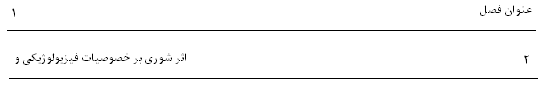
\includegraphics[width=.6\textwidth]{pages.png}
\caption{نمونه‌ای از شیوه‌ی صحیح قرارگیری مشخصات سرصفحه.}
\label{fig:header}
\end{figure}
			\begin{enumerate}[label=\Alph*:]
				\item سرصفحه (\lr{Header}) از صفحه‌ی دوم فصل اول شروع میشود و در صفحه‌ی اول هر فصل، قسمت سرصفحه حذف می‌شود. اول هر فصل باید \lr{break section} در بخش \lr{Page layout} استفاده شود تا سر فصل حذف شود و برای تکرار نشدن سرفصل‌ها در فصل‌های قبلی باید \lr{Link to previous} در بخش \lr{Design} استفاده شود.
				\item متن سرصفحه و شماره‌ی صفحه با قلم  \lr{BNazanin 12 Bold} نوشته شود. 
				\item صفحات سفید، سرصفحه ندارند. 
				\item صفحه‌ی اول فصل، پیوست، نمایه‌ها و واژه‌نامه، سرصفحه ندارند. 
				\item از صفحه‌ی فهرست تا شروع فصل اول، تمامی صفحات با حروف الفبای فارسی و در بالای صفحه، گوشه‌ی خارجی صفحه و به فاصله‌ی 5 سانتی‌متر از بالای كاغذ شماره‌گذاری ‌شود.
				\item از اولین صفحه‌ی فصل اول تا انتهای منابع، تمامی صفحات با اعداد1، 2، 3، و ... در بالای صفحه، گوشه‌ی خارجی صفحه و به فاصله‌ی 5 سانتی‌متر از بالای كاغذ شماره‌گذاری ‌شود.
			\end{enumerate}
			
		\section{نحوه‌ی نگارش}
			نرم‌افزار مورد استفاده برای نگارش پایان‌نامه،  \lr{Microsoft Word 2003} به بالا یا نرم‌افزار مناسب دیگر به تأیید كمیته‌ی تحصیلات تكمیلی دانشکده مربوطه می‌باشد. در صورت استفاده از برنامه \lr{Word}، توجه به نكات زیر ضروری است:  
			\begin{enumerate}%[label=\Alph*:]
				\item متن چکیده‌ی فارسی با قلم \lr{BNazanin 12} و کلمه «چکیده» در اولین خط با قلم \lr{BNazanin 12 Bold} در اول سطر درج شود. 
				\item متن چکیده‌ی انگلیسی با قلم \lr{Times New Roman 11} و کلمه \lr{Abstract} در اولین خط با قلم \lr{Time New Roman 11 Bold} در اول سطر درج شود. 
				\item متن مقدمه با قلم \lr{BNazanin 12} و کلمه «مقدمه» در اولین خط با قلم \lr{Bold  BNazanin 14} در اول سطر درج شود.
				\item متن اصلی پایان‌نامه باید روی دو طرف کاغذ \lr{A4} با قلم \lr{BNazanin 12} و با فاصله خطوط یکسان به صورت (\lr{Single}) نوشته شود. 
				\item در متن اصلی پایان‌نامه، لغات یا حروف انگلیسی (از جمله، منابع انگلیسی) با قلم \lr{Times New Roman 11} نوشته شود.
				\item عناوین فصل‌ها با قلم \lr{14 BNazanin Bold} نوشته شود.
				\item سطر اول تمامی پاراگراف‌های موجود در متن پایان‌نامه، بایستی $0.5$ سانتی‌متر تورفتگی داشته باشند. توجه داشته باشید که عنوان بخش‌ها یا زیر بخش‌ها نبایستی دارای تورفتگی باشند.
				\item قسمت‌های مختلف هر فصل با اعدادی نظیر 6-4- یا 6-4-2- مشخص میشود كه عدد 6 شماره‌ی فصل، عدد4 شماره‌ی بخش و عدد 2 شماره‌ی زیر بخش است. بخش‌های مختلف فصل‌ها با قلم \lr{BNazanin 13 Bold} و زیربخش‌های اول با قلم \lr{BNazanin 12 Bold}  و زیربخش‌های دوم با \lr{BNazanin 11 Bold} تایپ شود.
				\item تمامی شکل‌ها و جدول‌ها باید به ترتیب ظهور در هر فصل شماره‌گذاری شوند. مثلاً برای جدول‌های فصل 2، جدول 2-1، جدول 2-2 و ... برای جدول‌های فصل 3، جدول 3-1، جدول 3-2 و .... عنوان جدول‌ها در بالای آن‌ها و وسط صفحه و عنوان شکل‌ها در زیر آنها، وسط صفحه با قلم \lr{BNazanin 10 Bold}  نوشته شود. اعداد و متن داخل جدول با قلم \lr{BNazanin 10}   نوشته شود. اگر شکلی از مرجعی نقل شده باشد، لازم است مرجع آن در زیر شکل داخل پرانتز آورده شود.
				\item جدول‌هایی که در راستای طولی کاغذ تنظیم میشوند، باید طوری قرار گیرند که متن بالای آنها در سمت لبه‌ی پایان‌نامه واقع شود (درتمامی جدول‌ها خطوط عمودی باید حذف شود). شکل‌ها و جدول‌ها داخل متن و در نزدیکترین فاصله به محل ذکر شده، آورده شوند (حاشیه‌ی شکل‌ها حذف شود). هم‌چنین شکل‌هایی که در راستای طولی کاغذ تنظیم می‌شوند، باید طوری قرار گیرند که متن پایین آنها در سمت لبه‌ی پایان‌نامه قرار گیرد. 
				\item فرمول‌ها (در صورت نیاز به ارجاع) در هر فصل به‌طور جداگانه و به ترتیبی که ظاهر می‌شوند (مانند جدول‌ها و شکل‌ها) شماره‌گذاری می‌گردد (مانند 2-3، 2-4، 3-1 و ...).
				\item معادل انگلیسی لغات یا اصطلاحات فارسی که برای اولین‌بار به کار می‌رود به صورت زیرنویس (فقط برای یک‌بار) با قلم Times New Roman 10 در صفحه‌ی مربوط درج شود. (سعی شود در متن پایان‌نامه‌، از بکار بردن واژه‌های با الفبای انگلیسی خودداری شود). زیرنویس‌ها در هر صفحه با گذاردن شماره‌ی 1، 2 و ... در گوشه‌ی بالای آخرین کلمه در متن مشخص میشوند. زیر نویس باید به شکل زیر در زیر نویس آورده شود. \\
\begin{latin}
\footnotesize	$1$ Water use efficiency
\end{latin}
				\item لازم است در متن به تمامی منابعی كه مورد استفاده قرار می‌گیرند، اشاره شود. چنانچه در داخل متن از یك منبع مطلبی نقل شود، بلافاصله پس از ذكر نام نویسنده و یا در خاتمه‌ی جمله، پرانتزی باز شود و مرجع ذكر گردد. شیوه‌ی نامه‌ی نگارش منابع پیوست شده است (پیوست شماره‌ی \ref{app6}).
				
			\end{enumerate}

		حاشیه‌های صفحات مطابق نمونه‌ی شکل \ref{layout} ($4.5$ سانتیمتر فاصله از بالا و پایین و $4$ سانتیمتر از چپ و $5$ سانتیمتر از راست رعایت گردد (توجه: برای تنظیم این فاصله‌ها از حاشیه از طریق \lr{Page layout} وارد \lr{Page setup} شده و اعداد را با واحد سانتیمتر وارد کنید. در ضمن در همان صفحه در قسمت \lr{Multiple pages} کلمه \lr{mirror margin} را انتخاب کنید تا در صفحات زوج و فرد فاصله متن از حاشیه بیرونی $4$ سانتیمتر و از حاشیه درونی $5$ سانتیمتر شود (در \lr{Page setup} باید سایز (\lr{Size Letter}) انتخاب شود).
		
		\begin{figure}
	\centering
	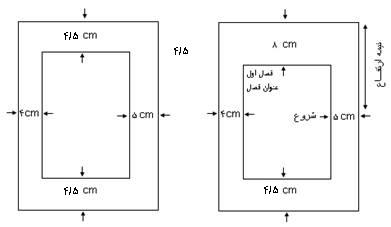
\includegraphics[width=.6\textwidth]{layout.png}
\caption{حاشیه‌ی صفحات.}
\label{layout}
\end{figure}
\section{نحوه‌ی صحافی پایان‌نامه}
	روی جلد مطابق یا پیوست شماره‌ی \ref{app1} تنظیم گردد، عطف آن مانند نمونه‌ی شکل \ref{atf} نوشته می‌شود.
	\begin{figure}
	\centering
	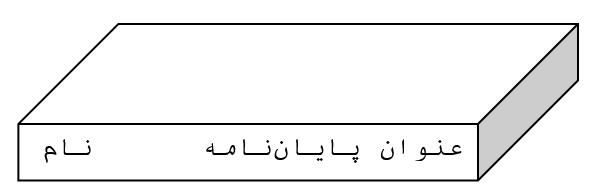
\includegraphics[width=.6\textwidth]{atf.png}
\caption{نمونه‌ای از شیوه‌ی صحیح \gls*{typeset} عطف.}
\label{atf}
\end{figure}
ابعاد پایان نامه بعد از صحافی، $23.5 \times 17$ (قطع وزیری) باید باشد. ابعاد سیاهه متن پایان‌نامه (از بالای متن سرصفحه تا پایین متن اصلی و عرض متن) $18.3 \times 12$ باید باشد. 
فاصله‌ی متن سرصفحه از حاشیه‌ی بالا $2.5$ سانتیمتر و فاصله‌ی متن اصلی از حاشیه‌ی پایین $2.7$ سانتیمتر، فاصله‌ی متن از حاشیه‌ی بیرونی $2$ سانتیمتر و از حاشیه‌ی درونی $3$ سانتیمتر باید باشد.  

رنگ جلد پایان‌نامه‌های کارشناسی‌ارشد کلیه رشته‌ها سورمه‌ای و رساله دکتری سبز یشمی می‌باشد. همچنین، اصل پایان‌نامه قبل از صحافی و پس از تایپ و آماده‌سازی به رؤیت مدیر تحصیلات تكمیلی دانشگاه یا معاون آموزشی دانشكده رسانیده شود و پس از مطابقت با ضوابط مصوب، تأییدیه صادر گردد.

